\documentclass[a4paper,11pt]{article}

% --- Encodage et Langue ---
\usepackage[utf8]{inputenc}
\usepackage[T1]{fontenc}
\usepackage[french]{babel}

% --- Mise en page et Typographie ---
\usepackage{geometry}
\geometry{margin=2.5cm, headheight=15pt}
\usepackage{microtype}
\usepackage{lmodern}

% --- En-têtes et pieds de page ---
\usepackage{fancyhdr}
\pagestyle{fancy}
\fancyhf{}
\renewcommand{\headrulewidth}{0pt}
\renewcommand{\footrulewidth}{0.4pt}
\fancyfoot[L]{\small\textcolor{primary}{\textit{Copyrights Jean-Christophe Le Lann -- Électronique Numérique}}}
\fancyfoot[R]{\small\textcolor{primary}{\thepage}}

% --- Mathématiques ---
\usepackage{amsmath, amssymb}
\usepackage{centernot}

% --- Couleurs et Boîtes ---
\usepackage{xcolor}
\definecolor{primary}{RGB}{0, 85, 150}      % Bleu technique
\definecolor{secondary}{RGB}{240, 248, 255} % Bleu très clair pour les fonds
\definecolor{solcolor}{RGB}{245, 250, 245}  % Vert très clair pour les solutions
\definecolor{solframe}{RGB}{60, 120, 60}    % Vert foncé pour les bordures de solution

\usepackage{tcolorbox}
\tcbuselibrary{skins}

% --- Tableaux professionnels ---
\usepackage{booktabs}
\usepackage{array}

% --- Affichage de code / binaire ---
\usepackage{listings}
\lstset{
    basicstyle=\ttfamily\small,
    backgroundcolor=\color{gray!5},
    frame=single,
    framerule=0.5pt,
    rulecolor=\color{gray!50},
    numbers=none,
    breaklines=true,
    keepspaces=true,
    columns=fullflexible
}

% --- Titres ---
\usepackage{titlesec}
\titleformat{\section}
  {\color{primary}\Large\bfseries}
  {\thesection}{1em}{}[\titlerule]

%==================================================================================
% --- Gestion des solutions (Mettre \solutionsfalse pour cacher les solutions) ---
%==================================================================================
\newif\ifsolutions
%\solutionstrue % <--- version prof
\solutionsfalse % <--- version étudiant
%==================================================================================

\newtcolorbox{notebox}{
  colback=secondary,
  colframe=primary,
  fonttitle=\bfseries,
  title=Notes et Conseils,
  arc=4pt,
  boxrule=0.8pt
}

\newtcolorbox{solbox}{
  colback=solcolor,
  colframe=solframe,
  fonttitle=\bfseries,
  title=Solution,
  arc=4pt,
  boxrule=0.8pt
}

% --- Titre du document ---
\title{\textcolor{primary}{\Huge\bfseries TD 1 -- Électronique Numérique}\\[0.5em] \Large Représentation des nombres et Logique combinatoire}
\author{}
\date{}

\begin{document}

\maketitle
\thispagestyle{fancy}   % <-- AJOUTER CETTE LIGNE pour forcer le copyright sur la 1ère page
\vspace{-2em}

\begin{notebox}
\begin{itemize}
    \item Le premier objectif de ce TD est de manipuler différentes représentations des \textit{nombres} et notamment de maîtriser les changements de base \textbf{sans calculatrice}.
    \item En dehors du TD, il est suggéré de vérifier que vous êtes suffisamment adroit pour les réaliser également \textit{avec} calculatrice ou à l'aide de votre langage de programmation préféré.
    \item Le second objectif est de se familiariser avec l'algèbre de Boole.
    \item \textit{Note : Tous les exercices ne seront pas nécessairement corrigés lors des séances de TD.}
\end{itemize}
\end{notebox}

\vspace{1em}

\part{Représentation des nombres}

\section{Compter en base 2 et base 16}
\begin{enumerate}
    \item Compter de 0 à 15 en binaire, puis en hexadécimal. \textit{(On conservera ces valeurs dans un tableau pour la durée de cette partie du TD)}

    \ifsolutions
    \begin{solbox}
    \begin{center}
      \renewcommand{\arraystretch}{1.2}
      \begin{tabular}{c c c}
        \toprule
        \textbf{Décimal} & \textbf{Binaire} & \textbf{Hexadécimal} \\
        \midrule
        0 & 0000 & 0 \\
        1 & 0001 & 1 \\
        2 & 0010 & 2 \\
        3 & 0011 & 3 \\
        4 & 0100 & 4 \\
        5 & 0101 & 5 \\
        6 & 0110 & 6 \\
        7 & 0111 & 7 \\
        8 & 1000 & 8 \\
        9 & 1001 & 9 \\
        10 & 1010 & A \\
        11 & 1011 & B \\
        12 & 1100 & C \\
        13 & 1101 & D \\
        14 & 1110 & E \\
        15 & 1111 & F \\
        \bottomrule
      \end{tabular}
    \end{center}
    \end{solbox}
    \fi

    \item Écrire les puissances de $2^n$ pour $n$ variant de 0 à 10. En déduire une valeur approchée de $\log_{10} 2$, puis $\log_{10} 5$. Avec un procédé similaire, trouver une valeur approchée de $\log_{10} 3$.

    \ifsolutions
    \begin{solbox}
    \begin{center}
      \renewcommand{\arraystretch}{1.2}
      \begin{tabular}{c c}
        \toprule
        $n$ & $2^n$ \\
        \midrule
        0 & 1 \\
        1 & 2 \\
        2 & 4 \\
        3 & 8 \\
        4 & 16 \\
        5 & 32 \\
        6 & 64 \\
        7 & 128 \\
        8 & 256 \\
        9 & 512 \\
        10 & 1024 \\
        \bottomrule
      \end{tabular}
    \end{center}
    \vspace{0.5em}
    On remarque que $2^{10} = 1024 \approx 10^3$. D'où :
    $$ \log_{10}(2^{10}) \approx \log_{10}(10^3) \implies 10 \log_{10} 2 \approx 3 \implies \log_{10} 2 \approx \frac{3}{10} = 0.3 $$
    (En réalité, $\log_{10} 2 \approx 0.301$ à $10^{-3}$ près. L'erreur est de 0.3\%).\\
    De même :
    $$ 5 = \frac{10}{2} \implies \log_{10} 5 = \log_{10} 10 - \log_{10} 2 \approx 1 - 0.3 = 0.7 $$
    Pour $\log_{10} 3$, on peut remarquer que $3^4 = 81 \approx 80 = 10 \times 2^3 \times 1$ (ou $3^2 \approx 10$). Une approximation courante utilise $3^4 \approx 10 \times 8 = 10 \times 2^3$ :
    $$ 4 \log_{10} 3 \approx 1 + 3 \log_{10} 2 \approx 1 + 3(0.3) = 1.9 \implies \log_{10} 3 \approx \frac{1.9}{4} = 0.475 $$
    (Valeur réelle $\approx 0.477$).
    \end{solbox}
    \fi

    \item Calculer la valeur décimale de $10101011_2$ en passant par les puissances de 2, puis en passant par les puissances de 16.

    \ifsolutions
    \begin{solbox}
    \begin{align*}
        10101011_2 &= 2^7 + 2^5 + 2^3 + 2^1 + 2^0 \\
                   &= 128 + 32 + 8 + 2 + 1 = \mathbf{171_{10}}
    \end{align*}
    En passant par l'hexadécimal (groupement par 4 bits : $1010$ et $1011$) :
    \begin{align*}
        1010\ 1011_2 &= \text{A}\text{B}_{16} \\
                     &= 10 \times 16^1 + 11 \times 16^0 \\
                     &= 160 + 11 = \mathbf{171_{10}}
    \end{align*}
    \end{solbox}
    \fi

    \item Écrire les puissances de $2^{-n}$ pour $n$ variant de 1 à 4.

    \ifsolutions
    \begin{solbox}
    \begin{center}
      \renewcommand{\arraystretch}{1.2}
      \begin{tabular}{c c}
        \toprule
        $n$ & $2^{-n}$ \\
        \midrule
        1 & 0,5 \\
        2 & 0,25 \\
        3 & 0,125 \\
        4 & 0,0625 \\
        \bottomrule
      \end{tabular}
    \end{center}
    \vspace{0.5em}
    Si on s'attribue 2 bits pour représenter (quantifier) une partie décimale, on a les équivalences suivantes :
    \begin{center}
      \begin{tabular}{c|c}
        \toprule
        Binaire & Décimal \\
        \midrule
        00 & 0,00 \\
        01 & 0,25 \\
        10 & 0,50 \\
        11 & 0,75 \\
        \bottomrule
      \end{tabular}
    \end{center}
    Pour 3 bits, on double la précision (pas de 0,125).
    \end{solbox}
    \fi
\end{enumerate}

\textit{Remarque :} Des nombres possédant une partie décimale sont transformés ici en de simples \textit{entiers}, en supposant que la position de la virgule est fixée à l'avance. Cette représentation est appelée \textbf{virgule fixe} (\textit{fixed-point}). Elle est très rapide à traiter par l'électronique, à coût matériel très faible, et est très utilisée en traitement du signal embarqué (DSP). À l'inverse, une représentation en \textbf{virgule flottante} est plus consommatrice de ressources (surface) et de temps, mais offre une plage dynamique et une précision beaucoup plus importantes (norme IEEE 754 traitée dans l'exercice 4).

\section{Conversions entre bases}
\begin{enumerate}
    \item Convertir le nombre $39_{10}$ en binaire.
    \ifsolutions
    \begin{solbox}
    On effectue les divisions successives par 2 :
    \begin{align*}
        39 &= 2 \times 19 + 1 \\
        19 &= 2 \times 9 + 1 \\
        9 &= 2 \times 4 + 1 \\
        4 &= 2 \times 2 + 0 \\
        2 &= 2 \times 1 + 0 \\
        1 &= 2 \times 0 + 1
    \end{align*}
    En lisant les restes de bas en haut : $39_{10} = \mathbf{100111_2}$.
    \end{solbox}
    \fi

    \item Convertir le nombre $(0,375)_{10}$ en binaire.
    \ifsolutions
    \begin{solbox}
    On effectue les multiplications successives par 2 :
    \begin{align*}
        0,375 \times 2 &= 0,75 \quad (\text{partie entière } 0) \\
        0,75 \times 2  &= 1,50 \quad (\text{partie entière } 1) \\
        0,50 \times 2  &= 1,00 \quad (\text{partie entière } 1)
    \end{align*}
    En lisant les parties entières de haut en bas : $0,375_{10} = \mathbf{0,011_2}$. (On remarque que $0,375 = 3 \times 0,125 = 3 \times 2^{-3}$).
    \end{solbox}
    \fi

    \item En déduire la représentation binaire du nombre $(39,125)_{10}$.
    \ifsolutions
    \begin{solbox}
    On combine les résultats précédents (en notant que $0,125 = 0,001_2$) :
    $$ (39,125)_{10} = \mathbf{100111,001_2} $$
    \end{solbox}
    \fi

    \item Convertir le nombre $(0,2)_{10}$ en binaire. Que remarquez-vous ?
    \ifsolutions
    \begin{solbox}
    On effectue les produits successifs :
    \begin{align*}
        0,2 \times 2 &= 0,4 \quad (0) \\
        0,4 \times 2 &= 0,8 \quad (0) \\
        0,8 \times 2 &= 1,6 \quad (1) \\
        0,6 \times 2 &= 1,2 \quad (1) \\
        0,2 \times 2 &= 0,4 \quad (0) \quad \leftarrow \text{On retombe sur le début !}
    \end{align*}
    On trouve $0,2_{10} = \mathbf{0,00110011\dots_2} = 0,\overline{0011}_2$.
    \textit{Remarque :} Une fraction décimale finie peut avoir une représentation binaire infinie périodique, ce qui explique les erreurs d'arrondi en informatique.
    \end{solbox}
    \fi

    \item Convertir $(345,158)_{10}$ en octal.
    \ifsolutions
    \begin{solbox}
    \textbf{Partie entière (divisions successives par 8) :}
    \begin{align*}
        345 / 8 &= 43 \quad \text{reste } \mathbf{1} \\
        43 / 8  &= 5 \quad \text{reste } \mathbf{3} \\
        5 / 8   &= 0 \quad \text{reste } \mathbf{5}
    \end{align*}
    $\implies 345_{10} = 531_8$\\
    \textbf{Partie décimale (multiplications successives par 8) :}
    \begin{align*}
        0,158 \times 8 &= 1,264 \quad (\mathbf{1}) \\
        0,264 \times 8 &= 2,112 \quad (\mathbf{2}) \\
        0,112 \times 8 &= 0,896 \quad (\mathbf{0}) \\
        0,896 \times 8 &= 7,168 \quad (\mathbf{7})
    \end{align*}
    $\implies 0,158_{10} \approx 0,1207_8$.\\
    Résultat final : $\mathbf{531,1207_8}$.
    \end{solbox}
    \fi

    \item Convertir $(389)_{10}$ en hexadécimal.
    \ifsolutions
    \begin{solbox}
    Divisions successives par 16 :
    \begin{align*}
        389 / 16 &= 24 \quad \text{reste } \mathbf{5} \\
        24 / 16  &= 1 \quad \text{reste } \mathbf{8} \\
        1 / 16   &= 0 \quad \text{reste } \mathbf{1}
    \end{align*}
    Résultat : $\mathbf{185_{16}}$ (ou \texttt{0x185}).
    \end{solbox}
    \fi

    \item Convertir $011001111011101_2$ en hexadécimal.
    \ifsolutions
    \begin{solbox}
    On groupe les bits par paquets de 4 en partant de la droite (on peut ajouter un 0 à gauche) :
    $$ 0110\ 0111\ 1011\ 1101_2 $$
    $$ \Downarrow $$
    $$ 6\quad 7\quad \text{B}\quad \text{D}_{16} $$
    Résultat : $\mathbf{67BD_{16}}$. \textit{(Note : le corrigé original indiquait 33DD, ce qui correspondait à un regroupement erroné. Le regroupement correct donne 67BD)}.
    \end{solbox}
    \fi

    \item Convertir $(10110001101011,1111)_2$ en octal.
    \ifsolutions
    \begin{solbox}
    On groupe les bits par paquets de 3 en partant de la virgule :
    \begin{lstlisting}
      010 110 001 101 011 . 111 100
        2   6   1   5   3 .   7   4
    \end{lstlisting}
    Résultat : $\mathbf{26153,74_8}$.
    \end{solbox}
    \fi

    \item Convertir $(10110001101011,111101)_2$ en hexadécimal.
    \ifsolutions
    \begin{solbox}
    On groupe les bits par paquets de 4 :
    \begin{lstlisting}
      0010 1100 0110 1011 . 1111 0100
         2    C    6    B .    F    4
    \end{lstlisting}
    Résultat : $\mathbf{2C6B,F4_{16}}$.
    \end{solbox}
    \fi

    \item Le nombre $101110001_2$ est écrit en BCD (décimal codé binaire). Convertir le nombre décimal obtenu en binaire pur. Combien de bits sont alors nécessaires ? Conclure.
    \ifsolutions
    \begin{solbox}
    En BCD, on groupe par 4 bits pour lire les chiffres décimaux :
    \begin{verbatim}
      0001  0111  0001
        1     7     1  => 171 en décimal
    \end{verbatim}
    Conversion de $171_{10}$ en binaire pur :
    $171 = 128 + 32 + 8 + 2 + 1 = 2^7 + 2^5 + 2^3 + 2^1 + 2^0$
    $\implies \mathbf{10101011_2}$.\\
    Il faut \textbf{8 bits} en binaire pur, contre \textbf{12 bits} (3 $\times$ 4) en BCD.\\
    \textit{Conclusion :} Le BCD est moins compact et moins efficace pour le calcul, mais il est très utile pour l'affichage direct sur des afficheurs 7 segments, car chaque digit est isolé.
    \end{solbox}
    \fi
\end{enumerate}

\section{Nombres signés en complément à 2}
\subsection*{Rappels}
Jusqu'ici, nous nous sommes intéressés aux nombres positifs. Il existe plusieurs manières de représenter un nombre négatif $n$. La manière la plus intuitive serait de dédier un bit (le plus à gauche) pour préciser le signe (ex: $0$ pour $+$, $1$ pour $-$). Malheureusement, cette représentation possède deux défauts majeurs : il existe deux représentations du zéro ($+0$ et $-0$) et il faut modifier l'algorithme d'addition.

Les architectes des ordinateurs ont retenu une autre représentation plus pratique : le \textbf{complément à 2}. C'est cette représentation qui régit le fonctionnement des \textit{unités arithmétiques et logiques} (ALU) des ordinateurs.

Avec $k$ bits, on peut représenter l'ensemble des nombres entiers dans l'intervalle :
$$ [-2^{k-1},\ \dots,\ 2^{k-1}-1] $$
Le complément à 2 d'un entier $n$ est obtenu par le calcul de la quantité $2^k - n$. On peut vérifier aisément que :
\begin{itemize}
    \item Le complément à 2 du complément à 2 d'un entier $n$ est $n$ lui-même.
    \item Le complément à 2 de zéro est zéro (on néglige la retenue qui dépasse la taille $k$ fixée).
\end{itemize}

On doit retenir la \underline{formule de passage en complément à 2} d'un nombre négatif $-X$ :
\begin{equation}
    -X = \overline{X} + 1
\end{equation}
La barre figurant au-dessus du $X$ signifie ``inversion de tous les bits'' (complément à 1). Si l'entier $n$ est codé sur $k$ bits ($s_{k-1}\dots s_0$) en complément à 2, sa valeur décimale est :
\begin{equation}
    n_{10} = -s_{k-1}2^{k-1} + \sum_{i=0}^{k-2} s_i2^i
\end{equation}

\subsection*{Exercices}
\begin{enumerate}
    \item Déterminer la plage des valeurs des entiers signés sur $k=4$ bits. Représenter ces valeurs en binaire. Quelles sont les représentations des valeurs extrêmes ? de 0, 1, et -1 ?
    \ifsolutions
    \begin{solbox}
    Avec $k=4$ bits, la plage est $[-2^{4-1},\ 2^{4-1}-1] = \mathbf{[-8,\ 7]}$.
    \begin{center}
      \renewcommand{\arraystretch}{1.1}
      \begin{tabular}{c c | c c}
        \toprule
        Décimal & Binaire (Cà2) & Décimal & Binaire (Cà2) \\
        \midrule
        -8 & \textbf{1000} & 0 & 0000 \\
        -7 & 1001 & 1 & 0001 \\
        -6 & 1010 & 2 & 0010 \\
        -5 & 1011 & 3 & 0011 \\
        -4 & 1100 & 4 & 0100 \\
        -3 & 1101 & 5 & 0101 \\
        -2 & 1110 & 6 & 0110 \\
        -1 & 1111 & 7 & 0111 \\
        \bottomrule
      \end{tabular}
    \end{center}
    \textbf{Points clés :}
    \begin{itemize}
        \item Les nombres positifs sont codés ``normalement''.
        \item Alors qu'en non-signé on pouvait compter jusqu'à $+15$ avec 4 bits, ici on est limité à $+7$.
        \item Les nombres qui présentent un `1' en MSB (Most Significant Bit) sont forcément négatifs \underline{dans cette représentation}.
        \item Le codage de la valeur $-1$ est $1111_2$.
    \end{itemize}
    \end{solbox}
    \fi

    \item Quel est le complément à 2 du nombre $8$, codé sur $6$ bits ? Utiliser la formule (1) et vérifier le résultat en appliquant la formule (2).
    \ifsolutions
    \begin{solbox}
    \textbf{Formule (1) :} On inverse tous les bits et on ajoute 1.
    $8_{10} = 001000_2$ (sur 6 bits) \\
    Inversion : $110111_2$ \\
    Ajout de 1 : $110111_2 + 1_2 = \mathbf{111000_2}$.

    \textbf{Formule (2) :} Vérification de la valeur de $111000_2$ :
    $$ -1 \times 2^5 + 1 \times 2^4 + 1 \times 2^3 + 0 + 0 + 0 = -32 + 16 + 8 = \mathbf{-8} $$
    Le résultat est cohérent.
    \end{solbox}
    \fi

    \item Soustraire : $91_{10} - 108_{10}$ en passant par le complément à 2.
    \ifsolutions
    \begin{solbox}
    Attention ! 91 et 108 peuvent se représenter sur 7 bits, mais pas $-108$. Il faut donc passer à \textbf{8 bits} pour éviter les débordements.
    \begin{align*}
        91_{10} &= 64 + 16 + 8 + 2 + 1 = 01011011_2 \\
        108_{10} &= 64 + 32 + 8 + 4 = 01101100_2 \\
        -108_{10} &= \overline{01101100} + 1 = 10010011 + 1 = 10010100_2
    \end{align*}
    Addition en complément à 2 :
    \begin{lstlisting}
        01011011  ( 91)
      + 10010100  (-108)
      -----------
        11101111
    \end{lstlisting}
    Vérification du résultat $11101111_2$ :
    $$ -2^7 + (2^6 + 2^5 + 2^3 + 2^2 + 2^1 + 2^0) = -128 + (64 + 32 + 8 + 4 + 2 + 1) = -128 + 111 = \mathbf{-17} $$
    Le calcul est correct ($91 - 108 = -17$).
    \end{solbox}
    \fi

    \item Écrire les nombres suivants en binaire sur 6 bits : $+24, +31, -24, -31$. Passez ensuite à 7 bits. Que remarquez-vous ?
    \ifsolutions
    \begin{solbox}
    \textbf{Sur 6 bits :}
    \begin{itemize}
        \item $+24 = 011000$
        \item $+31 = 011111$
        \item $-24 = \overline{011000} + 1 = 100111 + 1 = 101000$
        \item $-31 = \overline{011111} + 1 = 100000 + 1 = 100001$
    \end{itemize}
    \textbf{Sur 7 bits :}
    \begin{itemize}
        \item $+24 = 0011000$
        \item $+31 = 0011111$
        \item $-24 = \overline{0011000} + 1 = 1100111 + 1 = 1101000$
        \item $-31 = \overline{0011111} + 1 = 1100000 + 1 = 1100001$
    \end{itemize}
    \textit{Remarque :} On observe que le bit de signe se \textbf{propage} vers la gauche (c'est l'extension de signe). Pour passer d'une taille à une autre, il suffit de dupliquer le MSB.
    \end{solbox}
    \fi

    \item Soustraire : $1100\ 0101\ 0100\ 0000_2 - 101000\ 1111\ 1111_2 - 110\ 1111\ 1110_2 - 10\ 1110_2$.
    \ifsolutions
    \begin{solbox}
    \textit{Piège classique :} Si on ne tient pas compte du format et qu'on complémente ``mal'' (sans aligner les tailles), on obtient un résultat faux. Il faut ramener tous les opérandes à la même taille (ici, 16 bits minimum, mais 17 bits pour être sûr avec des signés).

    Valeurs décimales (pour vérification) : $50496 - 10495 - 1790 - 46 = 38165$.

    En se ramenant à une représentation \textbf{signée sur 17 bits} (pour gérer correctement le bit de signe de l'opérande positif initial de 16 bits) :
    \begin{lstlisting}
       0 1100 0101 0100 0000  (+50496)
     + 1 1101 0111 0000 0001  (-10495 en C2 sur 17 bits)
     + 1 1111 1001 0000 0010  (-1790 en C2 sur 17 bits)
     + 1 1111 1111 1101 0010  (-46 en C2 sur 17 bits)
     -----------------------
     1 0 1001 0101 0001 0101
    \end{lstlisting}
    La retenue de 18ème bit est ignorée. Le résultat sur 17 bits est $0\ 1001\ 0101\ 0001\ 0101_2$, qui vaut bien $\mathbf{38165_{10}}$.

    \textbf{Règle générale :} Pour additionner/soustraire des nombres signés, il faut les coder sur $n$ bits, où :
    $$ n = 1 + \max \Big( \lfloor \log_2(|x_1|) \rfloor + 1,\ \dots,\ \lfloor \log_2(|x_m|) \rfloor + 1 \Big) $$
    Ici, $n = 1 + \max(16, 14, 11, 6) = 17$ bits.
    \end{solbox}
    \fi
\end{enumerate}

\section{Norme IEEE 754}
\paragraph{Rappel : norme IEEE 754 (simple précision, 32 bits)}
Un flottant est codé par trois champs : 1 bit de signe $s$, 8 bits d'exposant $e$ et 23 bits de mantisse $m$.
La valeur représentée est, pour la plupart des nombres :
\[
V = (-1)^s \times 2^{\,e-127} \times (1 + m)
\]
où $m = \sum_{i=1}^{23} b_i 2^{-i}$ est la partie fractionnaire. L'exposant est représenté en excédent (biais) à $127$. La mantisse est toujours normalisée avec un $1$ implicite (gain de place), sauf pour les cas particuliers suivants :
\begin{itemize}
    \item si $e=255$ et $m=0$, alors $V = \pm\infty$ (selon $s$) ;
    \item si $e=255$ et $m \neq 0$, alors $V = \mathtt{NaN}$ (Not a Number) ;
    \item si $e=0$ et $m=0$, alors $V = \pm 0$ ;
    \item si $e=0$ et $m \neq 0$, il s'agit d'un nombre dénormalisé, dont la valeur est $V = (-1)^s \times 2^{-126} \times m$.
\end{itemize}

\paragraph{Exercice :} Représenter le nombre $238,4375$ dans sa représentation IEEE 754 (32 bits) en virgule flottante.

\ifsolutions
\begin{solbox}
\textbf{1. Conversion en binaire :}\\
Partie entière : $238_{10} = 128 + 64 + 32 + 8 + 4 + 2 = \mathbf{11101110_2}$\\
Partie décimale : $0,4375 = 0,25 + 0,125 + 0,0625 = 2^{-2} + 2^{-3} + 2^{-4} = \mathbf{0,0111_2}$\\
Donc : $238,4375_{10} = \mathbf{11101110,0111_2}$.

\textbf{2. Normalisation :}\\
On déplace la virgule pour obtenir un seul `1` avant la virgule :
$$ 11101110,0111_2 = 1,11011100111_2 \times 2^7 $$
L'exposant réel est $n = 7$.

\textbf{3. Codage des champs :}
\begin{itemize}
    \item \textbf{Signe ($s$) :} Le nombre est positif, donc $s = \mathbf{0}$.
    \item \textbf{Exposant ($e$) :} $e = n + 127 = 7 + 127 = 134_{10}$.\\
    $134_{10} = 128 + 4 + 2 = \mathbf{10000110_2}$.
    \item \textbf{Mantisse ($m$) :} On prend la partie fractionnaire après la virgule ($11011100111$) et on complète avec des zéros à droite pour atteindre 23 bits :\\
    $\mathbf{110\ 1110\ 0111\ 0000\ 0000\ 000_2}$.
\end{itemize}

\textbf{4. Assemblage final (32 bits) :}
\begin{lstlisting}
  S |    Exposant (8)   |          Mantisse (23)           |
  0 | 1 0 0 0 0 1 1 0 | 1 1 0 1 1 1 0 0 1 1 1 0 0 0 0 0 0 0 0 0 0 0 0 |
\end{lstlisting}
Soit en hexadécimal : $\mathbf{0x436E7000}$.
\end{solbox}
\fi

\part{Algèbre de Boole et Logique combinatoire}
Nous commençons par quelques manipulation élementaires autour de la minimisation d'expressions booléennes et leur mise en forme canonique, à l'aide de l'algèbre de Boole. Nous illustrons également la méthode des tableaux de Karnaugh qu'il faut voir comme une technique tabulée de minimisation astucieuse qu'il est intéressant de connaître pour de petits circuits. Nous poursuivons par la construction d'opérateurs matériels élémentaires : additionneurs, multiplexeurs, comparateurs.

\section{Quelques formulations booléennes}
Écrire sous la première forme canonique (somme de mintermes) les fonctions définies par les propositions suivantes :
\begin{enumerate}
    \item $F(a,b,c)=1$ si et seulement si aucune des variables $a,b,c$ ne prend la valeur 1.
    \item $F(a,b,c)=1$ si et seulement si au plus une des variables $a,b,c$ prend la valeur 0.
\end{enumerate}

\ifsolutions
\begin{solbox}
\centering
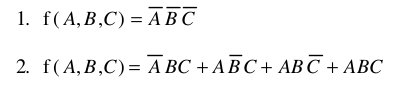
\includegraphics[scale=0.5]{./images/./te1-douillar-3.png}
%\captionof{figure}{Solutions des formulations booléennes}
\end{solbox}
\fi

\section{Minimisation d'expression booléennes}
Simplifier algébriquement les fonctions suivantes :
\begin{enumerate}
    \item $F = \overline{x}\overline{y} + xy + \overline{x}y$
    \item $F = (x+\overline{y})(x\overline{y}+z)z$
\end{enumerate}

\ifsolutions
\begin{solbox}
\begin{enumerate}
    \item $F = \overline{x}(\overline{y} + y) + xy = \overline{x}(1) + xy = \overline{x} + xy = (\overline{x} + x)(\overline{x} + y) = \mathbf{\overline{x} + y}$
    \item $F = (x+\overline{y})(x\overline{y}z + z) = (x+\overline{y})z(x\overline{y} + 1) = (x+\overline{y})z(1) = \mathbf{(x+\overline{y})z}$
\end{enumerate}
\end{solbox}
\fi

\section{Simplifications par tableaux de Karnaugh}
Simplifier, par la méthode des tableaux de Karnaugh, les fonctions booléennes suivantes. Dessiner le circuit correspondant et déterminer son chemin critique, en supposant que toutes les portes présentent un temps de propagation de 5 ns.

\subsection{K-map à 3 variables}
\begin{enumerate}
    \item $F(a,b,c) = \overline{a}\overline{b}c + \overline{a}b\overline{c} + ab\overline{c}$
    \item $F(a,b,c) = \overline{a}b\overline{c} + \overline{a}bc + ab\overline{c}$
    \item $F(a,b,c) = \overline{a}\overline{b}c + a\overline{b}\overline{c} + ab\overline{c}$, sachant que la valeur de $F$ pour les combinaisons $\overline{a}bc$ et $abc$ est indifférente (donc care $X$).
\end{enumerate}

\ifsolutions
\begin{solbox}
\begin{enumerate}
    \item $F(a,b,c) = \overline{a}\overline{b}c + b\overline{c}$
    \item $F(a,b,c) = \overline{a}b + b\overline{c} = b(\overline{a} + \overline{c})$
    \item $F(a,b,c) = \overline{a}c + a\overline{c} = a \oplus c$ (en utilisant les cares pour former des groupes de 2 optimaux).
\end{enumerate}
\end{solbox}
\fi

\subsection{K-map à 4 variables}
\begin{enumerate}
    \item $F(a,b,c,d) = \overline{a}b\overline{c}\overline{d} + \overline{a}b\overline{c}d + \overline{a}bcd + \overline{a}bc\overline{d}$
    \item $F(a,b,c,d) = \overline{a}\overline{b}\overline{c}d + \overline{a}\overline{b}cd + a\overline{b}\overline{c}d + a\overline{b}cd$
\end{enumerate}

\ifsolutions
\begin{solbox}
\begin{enumerate}
    \item En factorisant ou via le tableau, on isole $a=0$ et $b=1$ : $\mathbf{F = \overline{a}b}$
    \item On isole $b=0$ et $d=1$ : $\mathbf{F = \overline{b}d}$
\end{enumerate}
\end{solbox}
\fi

\section{Équations logiques de circuits de base}

\subsection{Additionneur}
\begin{enumerate}
    \item Établir la table de vérité d'un \textit{demi-additionneur} logique, puis les deux équations logiques associées : ce circuit additionne simplement 2 entrées booléennes $a$ et $b$ (donc \textit{sans retenue entrante}). Il calcule deux sorties : la somme $s$ et la retenue sortante $c_o$. Dessiner le circuit.

    \ifsolutions
    \begin{solbox}
    \begin{center}
      \renewcommand{\arraystretch}{1.2}
      \begin{tabular}{c c c c}
        \toprule
        $a$ & $b$ & $s$ & $c_o$ \\
        \midrule
        0 & 0 & 0 & 0 \\
        0 & 1 & 1 & 0 \\
        1 & 0 & 1 & 0 \\
        1 & 1 & 0 & 1 \\
        \bottomrule
      \end{tabular}
    \end{center}
    \vspace{0.5em}
    On trouve les équations suivantes :
    \begin{align*}
        s &= a \oplus b \\
        c_o &= a \cdot b
    \end{align*}
    \vspace{0.5em}
    \centering
    \fbox{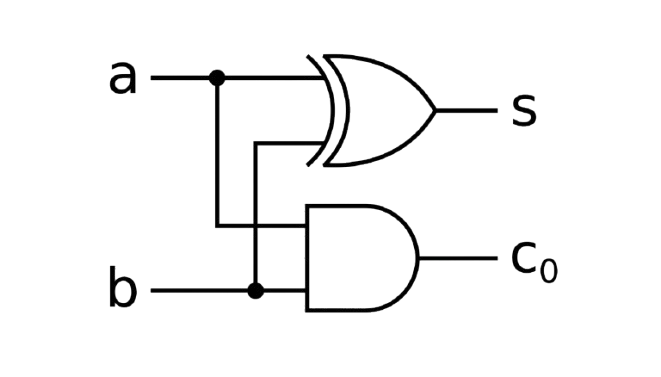
\includegraphics[scale=0.2]{./images/ha.png}}
    %\captionof{figure}{Circuit (netlist) du demi-additionneur 1 bit}
    \end{solbox}
    \fi

    \item Établir la table de vérité d'un \textit{additionneur complet} pour deux opérandes 1 bit. Ce dernier tient désormais compte d'une retenue entrante $c_i$. Établir les équations simplifiées des sorties, puis dessiner le circuit correspondant. Au préalable, on démontrera que : $\overline{x \oplus y} = x \oplus \overline{y}$.

    \ifsolutions
    \begin{solbox}
    Table de vérité :
    \begin{center}
      \renewcommand{\arraystretch}{1.2}
      \begin{tabular}{c c c c c}
        \toprule
        $a$ & $b$ & $c_i$ & $s$ & $c_o$ \\
        \midrule
        0 & 0 & 0 & 0 & 0 \\
        0 & 0 & 1 & 1 & 0 \\
        0 & 1 & 0 & 1 & 0 \\
        0 & 1 & 1 & 0 & 1 \\
        1 & 0 & 0 & 1 & 0 \\
        1 & 0 & 1 & 0 & 1 \\
        1 & 1 & 0 & 0 & 1 \\
        1 & 1 & 1 & 1 & 1 \\
        \bottomrule
      \end{tabular}
    \end{center}
    \vspace{0.5em}
    Formes brutes :
    \begin{align*}
        s &= \overline{a}\overline{b}c_i + \overline{a}b\overline{c_i} + a\overline{b}\overline{c_i} + abc_i \\
        c_o &= \overline{a}bc_i + a\overline{b}c_i + ab + \overline{c_i} + abc_i \quad \text{(Note: forme brute à simplifier)}
    \end{align*}
    Simplification :
    \begin{align*}
        s &= \overline{a}(b \oplus c_i) + a(b \oplus \overline{c_i}) \\
        c_o &= a \cdot b + c_i(a \oplus b)
    \end{align*}
    Démontrons que $\overline{x \oplus y} = x \oplus \overline{y}$ :
    \begin{align*}
        \overline{x \oplus y} &= \overline{x\overline{y} + \overline{x}y} \\
        &= (\overline{x} + y)(x + \overline{y}) \quad \text{(De Morgan)} \\
        &= \overline{x}x + \overline{x}\overline{y} + xy + y\overline{y} \\
        &= 0 + \overline{x}\overline{y} + xy + 0 \\
        &= x \oplus \overline{y}
    \end{align*}
    En posant $\alpha = b \oplus c_i$, on a pour la somme $s$ :
    \begin{align*}
        s &= \overline{a}\alpha + a\overline{\alpha} = a \oplus \alpha = a \oplus b \oplus c_i
    \end{align*}
    En résumé :
    \begin{align*}
        s &= a \oplus b \oplus c_i \\
        c_o &= a \cdot b + c_i(a \oplus b)
    \end{align*}
    \end{solbox}
    \fi

    \item Montrer qu'un additionneur complet ``1 bit'' peut réutiliser le demi-additionneur de la question 1.
    \ifsolutions
    \begin{solbox}
    \centering
    \fbox{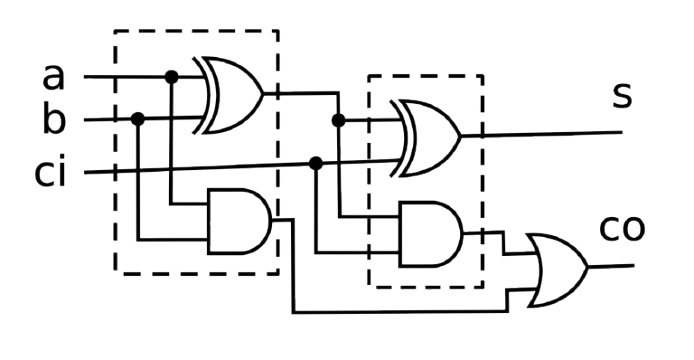
\includegraphics[scale=0.3]{./images/full_adder.png}}
    \fbox{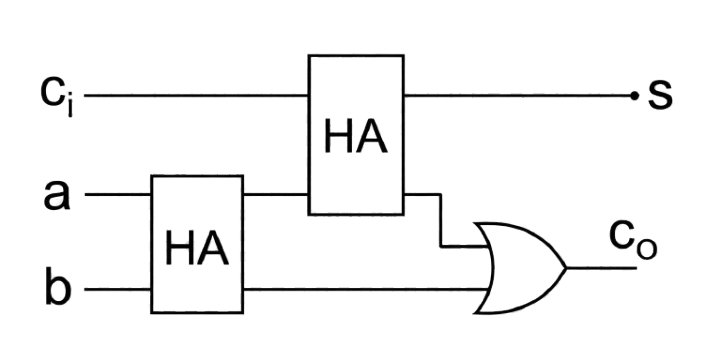
\includegraphics[scale=0.4]{./images/full_adder_ha.png}}
    %\captionof{figure}{Circuit de l'additionneur 1 bit complet (full-adder) et sa réalisation avec deux demi-additionneurs}
    \end{solbox}
    \fi

    \item Dessiner un additionneur 4 bits en réutilisant l'additionneur 1 bit.
    \ifsolutions
    \begin{solbox}
    On propose ci-dessous 2 solutions : la première ne permet pas l'utilisation de retenue entrante globale, tandis que la seconde utilise une telle retenue. La seconde solution est parfaitement régulière en terme d'aboutement, constituée de full-adders 1 bit en cascade.

    \vspace{1em}
    \centering
    \fbox{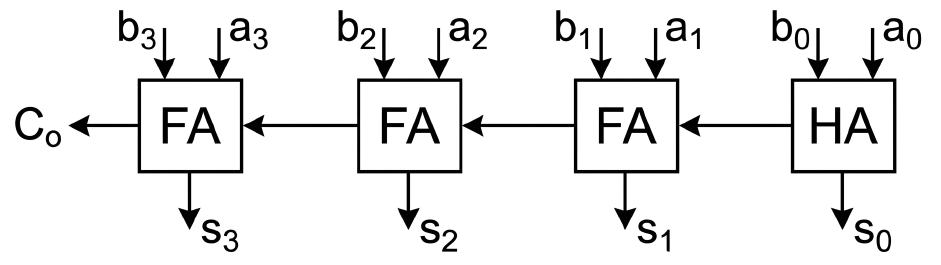
\includegraphics[scale=0.25]{./images/adder_4_wo_carry.png}}
    %\captionof{figure}{Additionneur 4 bits sans retenue entrante globale}

    \vspace{1em}
    \centering
    \fbox{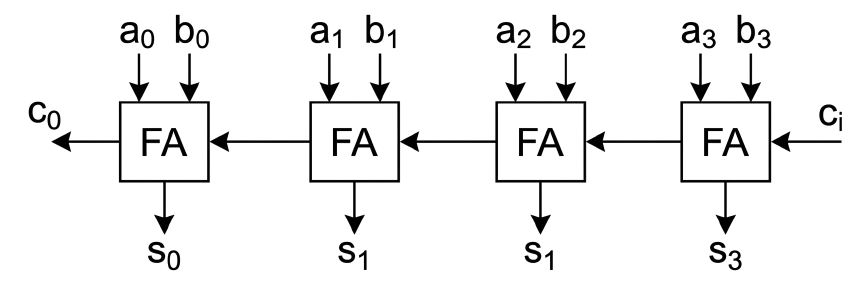
\includegraphics[scale=0.3]{./images/adder_4.png}}
    %\captionof{figure}{Additionneur 4 bits avec retenue entrante (Ripple Carry Adder)}
    \end{solbox}
    \fi

    \item Quel est le chemin critique de ce dernier circuit ? On rappelle que le chemin critique est le parcours le plus long entre une entrée et une sortie combinatoire. On le mesurera en nombre de portes logiques élémentaires traversées.
    \ifsolutions
    \begin{solbox}
    Dans la réalité, chaque porte logique est pré-caractérisée par des temps de traversée donnés par le constructeur (Intel, TSMC, etc.) et il faut sommer des \textit{temps}. L'exercice simplifie cela en comptant le nombre de portes ``abstraites''.\\
    Nommons les étages de 0 à 3. Deux cas distincts :
    \begin{enumerate}
        \item \textbf{Sans retenue entrante globale :} L'étage 0 a un chemin critique de 3 portes (2 demi-additionneurs + 1 OU). Les étages 1 à 3 ont un chemin critique de $c_{in}$ à $c_{out}$, soit 2 portes chacun. Total pour les 3 étages : $3 \times 2 = 6$. Chemin critique total : $\mathbf{3 + 6 = 9}$ portes.
        \item \textbf{Avec retenue entrante globale :} Le même raisonnement conduit à un chemin critique de \textbf{7 portes} traversées (le premier étage étant un full-adder complet dès le départ).
    \end{enumerate}
    \textit{Remarque :} structurellement, 9 portes existent dans le premier cas, créant un ``faux chemin critique'' si l'entrée est forcée à 0.
    \end{solbox}
    \fi

    \item Peut-on imaginer d'anticiper le calcul de la retenue ? Si oui, comment ?
\end{enumerate}

\subsection{Multiplexeur}
La fonction d'un multiplexeur est de sélectionner, grâce à un signal de contrôle, un signal d'entrée parmi plusieurs et de transmettre sa valeur sur une sortie unique.
\begin{enumerate}
    \item Dessiner le symbole communément admis pour représenter un multiplexeur à 2 entrées binaires (chacune codée sur 1 bit). On parle de multiplexeur "2 vers 1".
    \item Calculer l'équation d'un multiplexeur "2 vers 1" pour des entrées codées sur 1 bit.
    \item Lorsque les données d'entrées sont codées sur $n>1$ bits, chacun des bits du signal multiplexé suit évidemment un chemin similaire. Dessiner un tel multiplexeur à 2 entrées, pour $n=2$.
    \item Etablir la structure du multiplexeur à $m$ entrées, à l'aide de multiplexeurs.
    \item Calculer le nombre de couches logiques traversées pour un multiplexeur $m,n$ ("m vers 1" et dont les données sont codées sur $n$ bits).
\end{enumerate}

\ifsolutions
\begin{solbox}
On parle de multiplexeur 2-vers-1 (2-to-1 MUX).
\vspace{0.5em}
\centering
\fbox{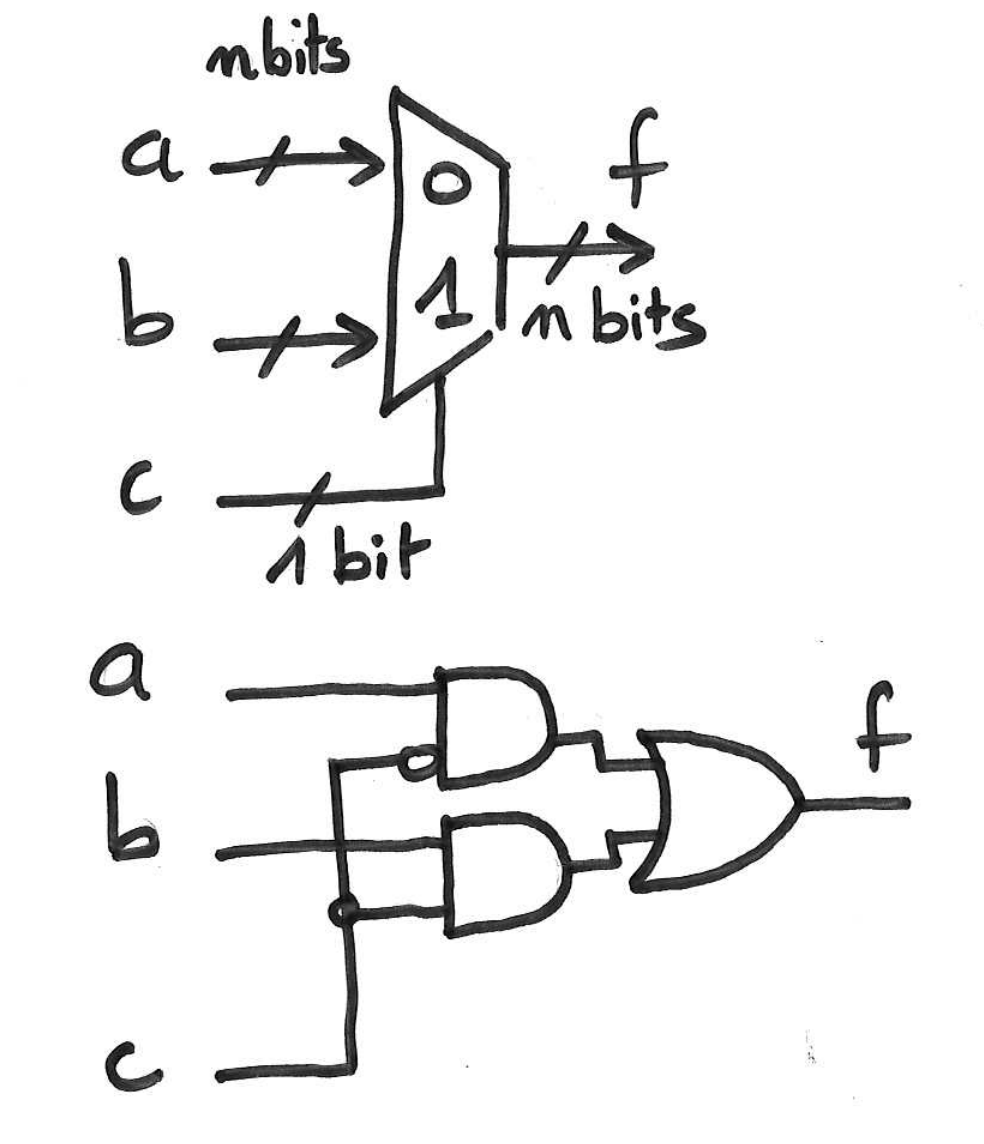
\includegraphics[scale=0.25]{./images/mux.png}}
%\captionof{figure}{Multiplexeur 2 vers 1, codé sur 1 bit : symbole et circuit}
\vspace{0.5em}
Pour $n$ bits, il suffit de mettre $n$ multiplexeurs 2-vers-1 en parallèle, tous pilotés par le même signal de sélection.
\end{solbox}
\fi

\subsection{Comparateur}
  Soit deux données $a$ et $b$ quelconques, encodées par deux variables booléennes générales $(a_{n-1},\dots,a_0) \in \mathcal{B}^n$ et $(b_{n-1},\dots,b_0) \in \mathcal{B}^n$.
\begin{enumerate}
  \item Démontrer que le résultat booléen $f$ de comparaison d'égalité entre les deux données vaut : $$f(a,b)=\prod_{i=0}^{i=n} \overline{a_{i} \oplus b_i} $$
  \item Dessiner la structure du comparateur matériel pour $n=4$.
\end{enumerate}

\section{Formes canoniques}
\noindent\textbf{Prérequis : Codage binaire et indexation des combinaisons booléennes}\\
Pour un système à $n$ variables logiques ordonnées, il existe $2^n$ combinaisons possibles de valeurs. Chaque combinaison peut être interprétée comme un nombre binaire, ce qui permet de lui associer de manière unique un indice entier compris entre $0$ et $2^n - 1$. Par exemple, pour trois variables ordonnées $(x, y, z)$, la combinaison de vérités $(1, 0, 1)$ est associée au mot binaire $101_2$, qui correspond à l'indice décimal $5$ : ce dernier pourra être évoqué comme le monôme $m_5$. Ce formalisme d'indexation numérique standardise la désignation de n'importe quel état du système et s'applique de manière générale en logique combinatoire, notamment pour l'organisation des tables de vérité, le référencement des cases d'un tableau de Karnaugh, etc.

\vspace{0.3cm}
\noindent\textbf{Formes canoniques et passage de l'une à l'autre}\\
La \textbf{première forme canonique} (ou Forme Normale Disjonctive, FND) est une somme de produits appelés mintermes ($m_i$), où chaque $m_i$ est le produit logique associé à la combinaison d'indice $i$ pour laquelle la fonction vaut $1$. À l'inverse, la \textbf{deuxième forme canonique} (ou Forme Normale Conjonctive, FNC) est un produit de sommes appelées maxterms ($M_i$), où chaque $M_i$ est la somme logique associée à la combinaison d'indice $i$ pour laquelle la fonction vaut $0$. Le passage d'une forme à l'autre exploite directement la complémentarité des indices au sein de l'ensemble des $2^n$ combinaisons. La fonction inverse $\bar{f}$ étant constituée des mintermes dont les indices sont absents de $f$, l'application de la double négation ($f = \overline{\bar{f}}$) et des lois de De Morgan permet de transformer la somme de ces mintermes manquants en un produit de maxterms de mêmes indices :
\begin{align*}
    f(x, y, z) &= m_1 + m_3 + m_5 \quad \text{(la fonction vaut 1 pour les indices 1, 3 et 5)} \\
    \bar{f}(x, y, z) &= m_0 + m_2 + m_4 + m_6 + m_7 \quad \text{(indices restants parmi les } 2^3 \text{ possibles)} \\
    f(x, y, z) = \overline{\bar{f}(x, y, z)} &= M_0 \cdot M_2 \cdot M_4 \cdot M_6 \cdot M_7 \quad \text{(par passage au dual via De Morgan)}
\end{align*}
Ainsi, commuter entre les deux formes canoniques revient simplement à inverser la nature de l'opérateur principal (somme ou produit) en basculant sur l'ensemble complémentaire des indices de l'univers des combinaisons.
% Toute fonction booléenne $F$ de plusieurs variables peut s'écrire sous deux formes spéciales, appelées \textit{formes canoniques} :
% \begin{itemize}
%     \item \textbf{Première forme (SOP)} : somme de produits (mintermes) de chaque variable \textit{ou de son complément}. On somme les produits pour lesquels la fonction vaut '1'.
%     \item \textbf{Seconde forme (POS)} : produit de sommes (maxtermes) de chaque variable \textit{ou de son complément}. On obtient cette forme de manière duale (pour les '0').
% \end{itemize}
\textit{Note : Ces formes ne sont pas simplifiées.}

Établir les deux formes canoniques des fonctions suivantes :
\begin{enumerate}
    \item $F_1 = xy + yz + xz$
    \item $F_2 = x + yz + \overline{y}\overline{z}t$
\end{enumerate}

\ifsolutions
\begin{solbox}
\centering
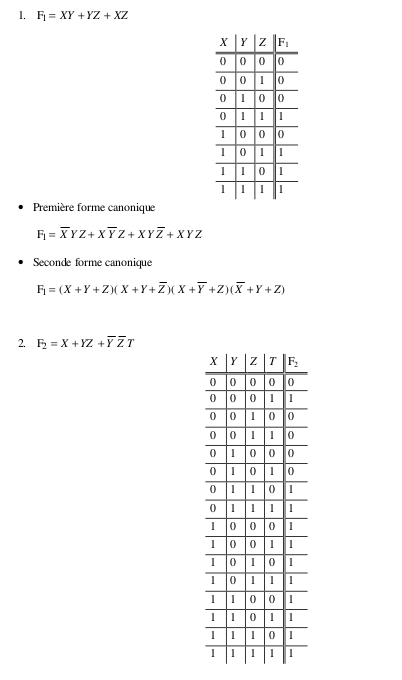
\includegraphics[scale=0.8]{./images/./te1-douillar-1.png}
%\captionof{figure}{Solution pour $F_1$}
\vspace{1em}
\centering
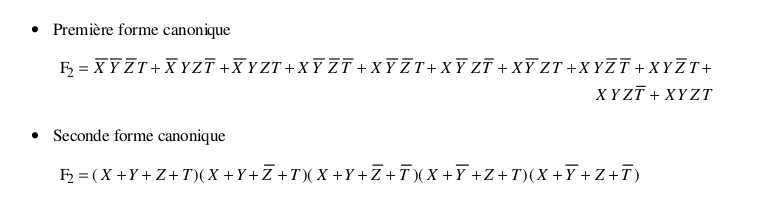
\includegraphics[scale=0.5]{./images/./te1-douillar-2.png}
%\captionof{figure}{Solution pour $F_2$}
\end{solbox}
\fi

\newpage



\newpage

% \section{Différentes utilisations du OU exclusif}
% \begin{enumerate}
%     \item Rappeler la table de vérité du OU exclusif, ainsi que son symbole (américain).
%     \item Dessiner la fonction OU-exclusif à partir de portes logiques ET, OU et NON.
%     \item Le OU-exclusif possède de nombreuses propriétés intéressantes. Compléter les énoncés suivants :
%     \begin{enumerate}
%         \item Sa sortie vaut 1 si exactement une des entrées vaut 1 : $x \oplus y = ?? + ??$
%         \item On peut le considérer comme un comparateur d'égalité pour 1 bit : $x \oplus y = \text{SI } (x==y) \text{ ALORS ? SINON ?}$
%         \item On peut le considérer comme un inverseur conditionnel : $x \oplus y = \text{SI } (?) \text{ ALORS ? SINON ?}$
%         \item On peut enfin le considérer comme un additionneur modulo 2.
%     \end{enumerate}
% \end{enumerate}
%
% \ifsolutions
% \begin{solbox}
% \begin{enumerate}
%     \item $x \oplus y = x\overline{y} + \overline{x}y$
%     \item $x \oplus y = \text{SI } (x==y) \text{ ALORS } 0 \text{ SINON } 1$ (C'est l'inverse de l'égalité, c'est un détecteur de différence).
%     \item $x \oplus y = \text{SI } (y==1) \text{ ALORS } \overline{x} \text{ SINON } x$. (Si $y=0$, $x \oplus 0 = x$ ; si $y=1$, $x \oplus 1 = \overline{x}$).
% \end{enumerate}
% \end{solbox}
% \fi
%


\section{Vu-mètre}
On se propose de réaliser un ``contrôleur de vu-mètre'' : c'est un dispositif qui permet de visualiser une grandeur numérique (un volume sonore par exemple) au moyen d'une barrette lumineuse qui s'étire plus ou moins en fonction de la grandeur.

\begin{enumerate}
    \item Schématiser le principe d'ensemble dans le cas où la grandeur à visualiser est codée sur 3 bits.
    \item À partir du tableau de Karnaugh, trouver une réalisation possible.
    \item On suppose que l'on dispose désormais d'un composant complexe de décodage (un décodeur 3 vers 8). Rappeler la table de vérité de ce circuit. Utiliser alors ce décodeur pour proposer une nouvelle réalisation.
\end{enumerate}

\ifsolutions
\begin{solbox}
\textbf{Attention :} lorsqu'on envoie le code \texttt{000}, on ne veut \textit{aucune} LED allumée. Quand on envoie le code \texttt{111} (7), on veut voir 7 LEDs allumées, numérotées de $L_0$ à $L_6$ (et non 8).

\textbf{Table de vérité du Vu-mètre :}
\begin{center}
  \renewcommand{\arraystretch}{1.2}
  \begin{tabular}{c c c c c c c c c c}
    \toprule
    $e_2$ & $e_1$ & $e_0$ & $L_0$ & $L_1$ & $L_2$ & $L_3$ & $L_4$ & $L_5$ & $L_6$ \\
    \midrule
    0 & 0 & 0 & 0 & 0 & 0 & 0 & 0 & 0 & 0 \\
    0 & 0 & 1 & 1 & 0 & 0 & 0 & 0 & 0 & 0 \\
    0 & 1 & 0 & 1 & 1 & 0 & 0 & 0 & 0 & 0 \\
    0 & 1 & 1 & 1 & 1 & 1 & 0 & 0 & 0 & 0 \\
    1 & 0 & 0 & 1 & 1 & 1 & 1 & 0 & 0 & 0 \\
    1 & 0 & 1 & 1 & 1 & 1 & 1 & 1 & 0 & 0 \\
    1 & 1 & 0 & 1 & 1 & 1 & 1 & 1 & 1 & 0 \\
    1 & 1 & 1 & 1 & 1 & 1 & 1 & 1 & 1 & 1 \\
    \bottomrule
  \end{tabular}
\end{center}

\textbf{Simplification (K-map) :}
\begin{align*}
    L_0 &= e_2 + e_1 + e_0 \\
    L_1 &= e_2 + e_1 \\
    L_2 &= \overline{e_2}e_1 + e_2\overline{e_1}e_0 \quad \text{(ou forme équivalente)} \\
    L_3 &= e_2 \\
    L_4 &= e_2 e_1 + e_2 \overline{e_1} e_0 \\
    L_5 &= e_2 e_1 \\
    L_6 &= e_2 e_1 e_0
\end{align*}

\textbf{Réalisation avec un décodeur 3 vers 8 :}\\
La sortie $C_i$ d'un décodeur s'allume (vaut 1) uniquement lorsque la valeur binaire d'entrée correspond à $i$.
\begin{center}
  \renewcommand{\arraystretch}{1.2}
  \begin{tabular}{c c c c c c c c c c c}
    \toprule
    $e_2$ & $e_1$ & $e_0$ & $C_0$ & $C_1$ & $C_2$ & $C_3$ & $C_4$ & $C_5$ & $C_6$ & $C_7$ \\
    \midrule
    0 & 0 & 0 & 1 & 0 & 0 & 0 & 0 & 0 & 0 & 0 \\
    0 & 0 & 1 & 0 & 1 & 0 & 0 & 0 & 0 & 0 & 0 \\
    0 & 1 & 0 & 0 & 0 & 1 & 0 & 0 & 0 & 0 & 0 \\
    0 & 1 & 1 & 0 & 0 & 0 & 1 & 0 & 0 & 0 & 0 \\
    1 & 0 & 0 & 0 & 0 & 0 & 0 & 1 & 0 & 0 & 0 \\
    1 & 0 & 1 & 0 & 0 & 0 & 0 & 0 & 1 & 0 & 0 \\
    1 & 1 & 0 & 0 & 0 & 0 & 0 & 0 & 0 & 1 & 0 \\
    1 & 1 & 1 & 0 & 0 & 0 & 0 & 0 & 0 & 0 & 1 \\
    \bottomrule
  \end{tabular}
\end{center}

\end{solbox} % cesure nécessaire pour mise en page !

\begin{solbox}
On remarque que $L_k$ doit être allumée pour toutes les valeurs d'entrée strictement supérieures à $k$. Ainsi :
\begin{align*}
    L_0 &= C_1 + C_2 + C_3 + C_4 + C_5 + C_6 + C_7 \\
    L_1 &= C_2 + C_3 + C_4 + C_5 + C_6 + C_7 \\
    L_2 &= C_3 + C_4 + C_5 + C_6 + C_7 \\
    &\vdots \\
    L_5 &= C_6 + C_7 \\
    L_6 &= C_7
\end{align*}
On peut réaliser cela en cascade avec des portes OU, ce qui est très élégant et modulaire. Seul le cas du zéro ($L_0$ éteinte quand $C_0=1$) est géré naturellement car $C_0$ n'est pas inclus dans la somme de $L_0$.

\vspace{0.5em}
\centering
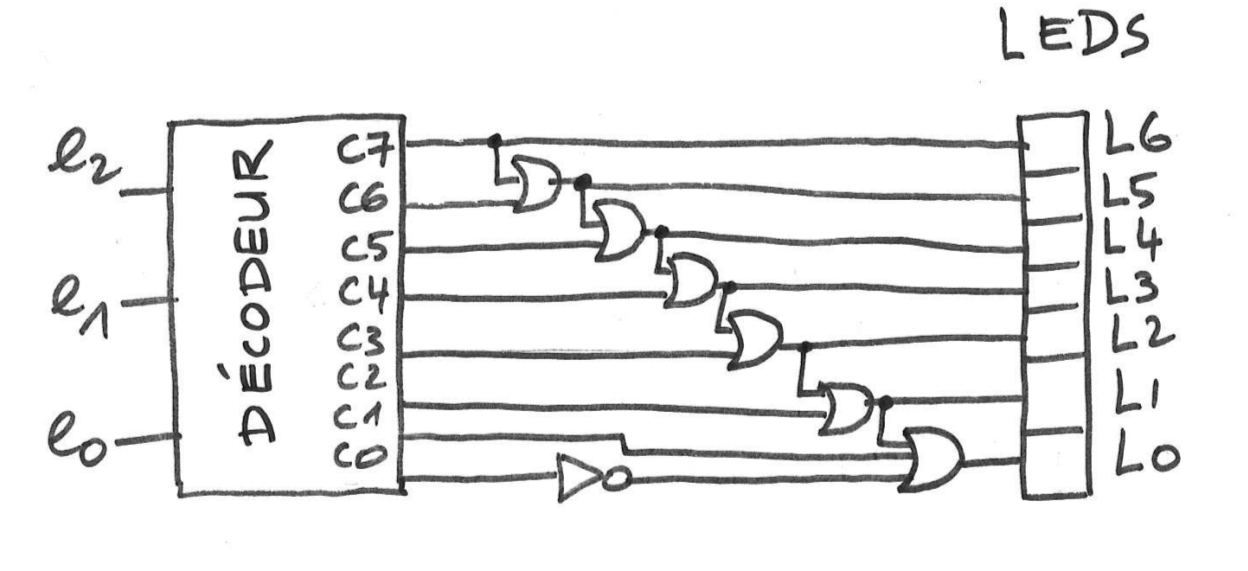
\includegraphics[scale=0.3]{./images/./vumetre-2015.png}
%\captionof{figure}{Réalisation du Vu-mètre à l'aide d'un décodeur et de portes OU}
\end{solbox}
\fi
\section{Le jeu des cambrioleurs}
Le principe du jeu \footnote{Le jeu est inspiré du jeu "Dix de Chute" des années 70.} est le suivant : un jeton est introduit par le joueur en haut du dispositif. Le but est de faire circuler ce jeton dans le dispositif, jusqu'à ce qu'il apparaisse en sortie. Dans l'intervalle, le jeton peut rester coincé à différents endroits (ou ``niveaux'') : seul un code secret correctement introduit à cet endroit permet au jeton de continuer son parcours. Sinon, l'utilisateur voit le code d'erreur \texttt{0xDEAD} apparaître en sortie. Chaque code secret, associé au niveau $i$, est codé sur 4 bits.

\begin{enumerate}
    \item Imaginer un circuit combinatoire qui simule ce jeu. On utilisera pour cela différents circuits connus : multiplexeurs et comparateurs. Enrichir votre circuit avec d'autres circuits combinatoires afin d'indiquer le nombre de niveaux franchis correctement.
    \item Sachant que l'on peut envoyer 1 million de codes par seconde, combien de temps faudrait-il, au pire cas, pour tester toutes les combinaisons possibles, dans le cas où le nombre de niveaux est 9 ? Refaites le calcul pour des codes sur 5 bits.
\end{enumerate}
\textit{Cet exercice ne nécessite pas de formules complexes, mais une réflexion architecturale.}

\ifsolutions
\begin{solbox}
\textbf{1. Architecture :}\\
Le but est de manipuler des circuits pour réaliser un ``chemin de données''. On choisit de représenter le jeton par un vecteur de bits de taille $n=16$ (à cause du code \texttt{0xDEAD}).\\
À chaque niveau, un comparateur vérifie si le code d'entrée correspond au code secret. La sortie du comparateur pilote un multiplexeur : si le code est bon, le jeton actuel passe au niveau suivant ; sinon, la valeur \texttt{0xDEAD} est injectée et propagée jusqu'à la sortie. Un compteur peut être incrémenté à chaque comparaison réussie.

\vspace{0.5em}
\centering
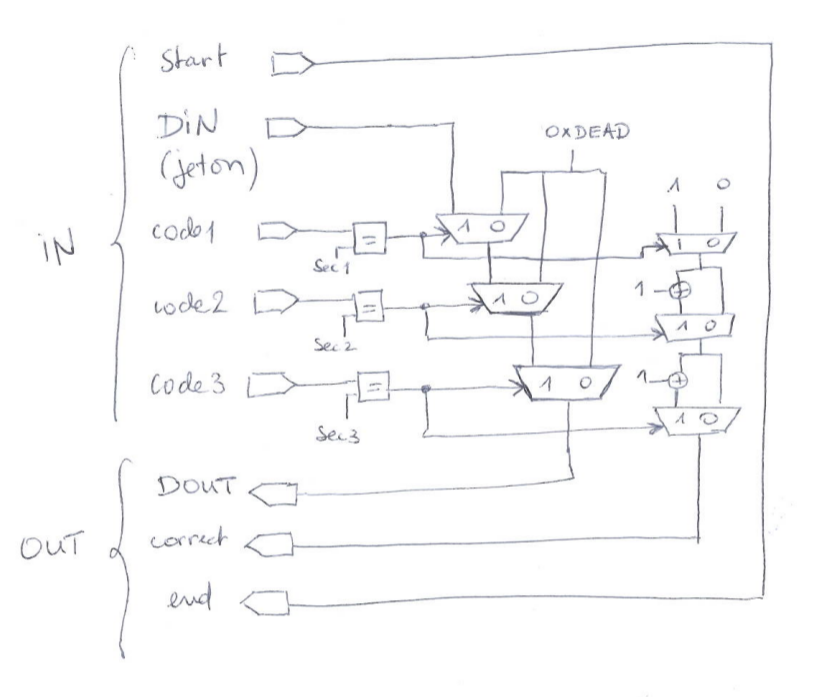
\includegraphics[scale=0.5]{./images/./cambrioleur.png}
%\captionof{figure}{Schéma de principe du jeu des cambrioleurs}
\vspace{0.5em}

\textbf{2. Calcul de complexité :}\\
Pour 9 niveaux avec des codes de 4 bits : il y a $(2^4)^9 = 2^{36}$ combinaisons à tester.\\
À $10^6$ tests/seconde, le temps au pire cas est :
$$ \frac{2^{36}}{10^6} \approx 68\,719 \text{ secondes} \approx \mathbf{19 \text{ heures}} $$
Pour des codes sur 5 bits : $(2^5)^9 = 2^{45}$ combinaisons.
$$ \frac{2^{45}}{10^6} \approx 35\,184\,372 \text{ secondes} \approx \mathbf{407 \text{ jours}} $$
\end{solbox}
\fi
\end{document}
